\documentclass{mcmthesis}
\mcmsetup{CTeX = false,   % 使用 CTeX 套装时,设置为 true
        tcn = 2113265, problem = C,    %队号和题号
        sheet = true, titleinsheet = true, keywordsinsheet = true,
        titlepage = false, abstract = true}
\usepackage{newtxtext}%\usepackage{palatino}
\usepackage{lipsum}
\usepackage{graphicx}
\usepackage{subfigure} 
\usepackage{float}   %{H}
\usepackage{listings}
\usepackage{parskip}
\setlength{\parindent}{0cm}
\lstset{%
	breaklines=true
}
\setcounter{tocdepth}{3}
\title{Bumblebee prediction based on LSTM network and VGG19 pre-trained convolutional neural network}%论文标题
\author{\small \href{https://www.latexstudio.net/}
  {\includegraphics[width=7cm]{mcmthesis-logo}}}
\date{\today}
\begin{document}
\begin{abstract}%========================%摘要(和关键词一起不要超过一页)
	
As an invasive species, Vespa mandarine appears in Washington State. Enthusiastic citizens provide sighting reports for the government's follow-up investigations while the accuracy of sighting reports is poor. In order to efficiently and accurately use these data and predict the future distribution of V.M, we combine models such as LSTM network,VGG19 pre-trained convolutional neural network and so on. The solutions will contribute to prevent the harmful effects of invading wasps on the environment and economic development in advance, which is of practical significance.

For \textbf{problem one}, It is a predictive problem. We firstly expand the sample data by interpolation. And then we propose a model reflecting the relationship between the spatial position and temporal change of wasps based on the LSTM algorithm. Experiments show that our model has $ 62\% $ accuracy. Finally,we simulate the potential distribution of wasps in the future based on this model. It provides a theoretical basis for wasp control.

For \textbf{problem two}, we construct a wasp classification model. Due to the large difference in the number of positive and negative samples, we use various methods to expand the data, such as translation, rotation and adding noise. Meanwhile, the non-wasp data is down-sampled. Next,on a small sample of wasp data,we conduct a  classification model of wasp image based on the pre-trained VGG convolutional neural network by transfer learning.  Our model can achieve an accuracy of more than $ 92\% $ in the experiment so that it can effectively detect wasps with small errors.

For \textbf{problem three}, we start with a new string consisting of 50 most frequent words in the Negative ID sample and call the new one the Negative dictionary string.Second. TFIDF is used to extract the text word vector from the target report. We calculate the similarity between the target text and Negative dictionary string and compare similarity with the threshold. Finally, combined with the image information results in Model 2, three response levels are constructed to achieve a more objective response. We test Unprocessed and unverified samples in the data.Experiments show that our method can effectively divide response levels and greatly save time of manual judgment.

For \textbf{problem four}, we consider that deep learning model training often requires a large amount of data, so we combine the temperature situation and the life habits of wasps to make statistics on the report data generated every month. On the premise of ensuring effective data volume, we believe that the model should be updated as soon as possible.After analyzing the data, we find that the reports are mainly produced from April to October, especially the peak in August to September. Therefore, we conclude that updates should be made between August and September every year, and the frequency of updates should be once a year.

For \textbf{problem five}, we think of it as a concrete application of the previous model. Once there are no more primary and secondary responses, the pest is eradicated.

\begin{keywords}%===========================================%关键词
Long short term memory(LSTM) network; VGG19 pre-trained CNN;Word cloud
\end{keywords}
\end{abstract}
\maketitle
\tableofcontents%===========================================%自动生成目录
\newpage
%===========================================================%正文

%--------------------------------------------------------------------
\section{Introduction}
\subsection{Problem Background}
\hspace*{\fill}

The destruction of biodiversity caused by the increasing species invasion has been the focus of recent years. In addition to being one of the greatest threats to biodiversity and ecosystems, biological invasions have also caused enormous losses to the global economy. Invasive species have adverse effects on neocolonial regions, such as impoverishing native species assemblages in terrestrial and aquatic habitats, and decreasing key insects that supply biological control and pollution services. Due to their impact on local honey bee colonies, and possible negative human health effects from stings and their allergenic effects. The increase in invasive species and their impact on biodiversity and ecosystems raise a number of management and control issues.

A typical example is the emergence of Asian giant wasps on Vancouver Island in Canada and Washington State in the US, severely injuring local species in succession. Bumblebees of the genus Vespa are known to have serious negative effects on honey bee colonies, hunting foragers while attacking hives. These hybrid bumblebees live in social colonies established by female bees and can produce colonies in areas of human modification such as agricultural or urban landscapes. Because its nest is usually built underground, it is very hidden and difficult to find. At the same time, its appearance and life cycle similar to those of local bees interfere with human judgment.

It is recognized to prevent the establishment and further spread of invasive species. In order to avoid harmful economic and environmental consequences, Washington State plans to further investigate and study the specific scope of the invasion through the hotline and the information posted on the website by enthusiastic citizens, and then use limited resources to guide future eradication attempts. Figure 1 shows a simplified detection location map of Asian bumblebee. The result is a large number of false sights and only a few confirmed sights, which is not optimistic.

\begin{figure}[H]
	\centering
	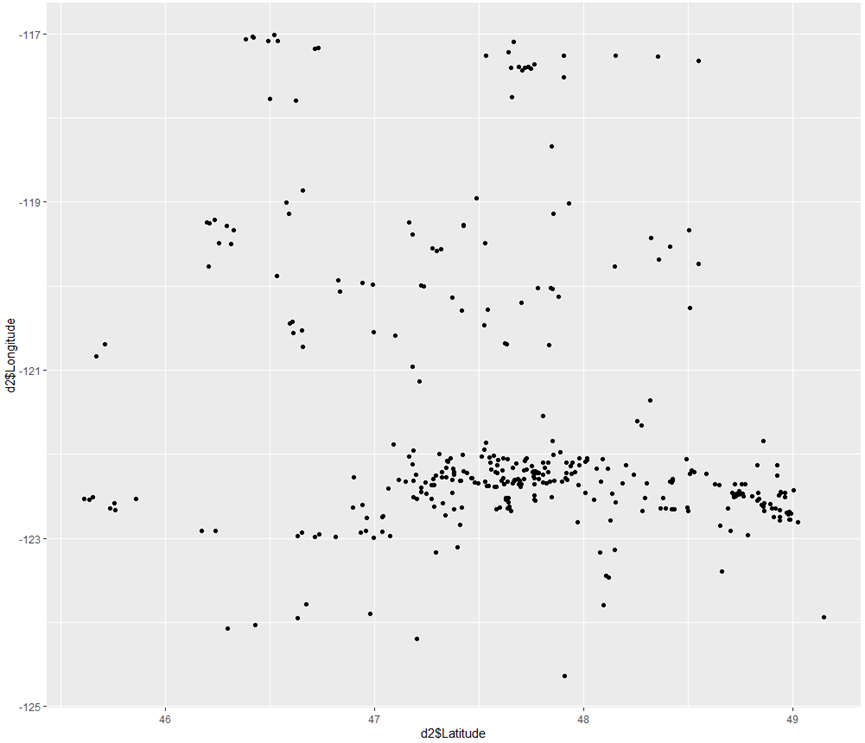
\includegraphics[width=0.55\textwidth]{screenshot002}
	\caption{Map depicting Asian Giant Hornet Detections, as well as Hornet Watch and Public Sitting locations.(After the simplification)}
	\label{fig:screenshot002}
\end{figure}

\subsection{Restatement of the Problem}  
Considering the background information and restricted conditions identified in the problem statement, we need to solve the following problems:
\begin{enumerate}
	\item[\textbf{Problem 1}]Reliably predict the potential spread of the Hornet in North America in the future, and point out the accuracy of the forecast. Namely,solve and discuss whether it is possible to predict the spread of this pest over time.
	\item[\textbf{Problem 2}]Only use the data set and image files provided in the attachment to generate a predictive model. This model can point out the possibility that eyewitnesses will mistake the bee they see for the Asian Hornet, which is the possibility of anticipating misclassification.
	\item[\textbf{Problem 3}] Apply the established model to analyze the information provided by the witnesses, and explain that the events selected by the model that should be given priority investigation privileges are most likely to be the correct working principles of the witnesses.
	\item[\textbf{Problem 4}]When there are more reports of sightings, determine how to update the model to accommodate the analysis of the latest report, and determine the frequency of updating the model.
	\item[\textbf{Problem 5}] Through the analysis of the model created, it is indicated out under what situation and evidence that the pests were eradicated by Washington State.
\end{enumerate}
\hspace*{\fill}
\subsection{Literature Review}
Prior to this, the Asian Hornet was mainly anticipated based on objective nat-ural factors. 

First from the point of view of the abiotic part , many scholars have analyzed and studied different ecosystem factors related to the Asian Hornet. Norderud , Powell $ \& $ Peterson(2021) estimate for Asian Hornet queens to overwinter and colonize nests, density and distribution of apiaries based on climate and habitat suitability. In addition, by analyzing the organ-isms related to the Asian Hornet ,Gonzalez et al. (2021) thought the North American Asian bumblebee habitat is expected to roughly coincide with the highest honey production areas. This provides prey for the Asian Hornet. Futhermore, many people have proposed corresponding prediction methods and models. For example, based on the environmental factors,Jin and Li(2015) provided forecasting methods, such as experiential forecasting, ex-perimental forecasting and statistical forecasting. According to Morgane et al.(2018), The SDMS predicts the potential range of invasive species, using the Asian bumblebee as an example. The accuracy needs to be improved. However, when data is obtained, it is likely that its image will need to be clas-sified with other images of wasps that may be confusing. Kwon and Lee (2020)gave the recognition score and classification accuracy of the fused wasp image based on the Deep Convolutional Neural Networks (DCNN) AlexNet algorithm.

\hspace*{\fill}
\section{Preparation of the Models}

\subsection{Assumptions and Justifications}
To simplify our model and eliminate the complexity, we make the following main assumptions in this literature. All assumptions will be re-emphasized once they are used in the construction of our model.
\begin{enumerate}
	\item \textbf{We assume that disregarding the influence of specific external factors such as climate.}
	
	Only the combined effect of all influences is recognized in the forecast.
	\item \textbf{We assume that the past of things will continue into the future as well.}
	
	First, the development of things generally follows objective laws.The factors that influence the distribution of Asian bumblebees will remain almost the same as  the past ones, so that their distribution can continue to follow past patterns.In other words, bumblebee distribution will not change in sudden jumps in the future, but in relatively small steps.Second, past and present phenomena may indicate trends in the development and change of present and future activities.
	\item \textbf{We assume that the queen bee is inactive in winter.}
	
	Like other wasps, Asian bumblebees have a biological clock of one year. During the cold winter, the new queen leaves the nest and spends the winter in the soil. The only survivor waiting for spring is the wintering queen bee. In the spring, the queen bee is active and builds nests. This indicates that the queen is inactive during the winter.
	\item \textbf{We assume that the flying distance of the queen bee during breeding is 30km.}
	
	We assume that the past of things will continue into the future as well.
	
\end{enumerate}
\hspace*{\fill}
\subsection{Notions and Symbol Description}
We will define the following variables here as they are used throughout our paper.
\begin{table}[H]
\centering
	\begin{tabular}{cc}
		\toprule[1.5pt]
		Symbols& Definitions\\
		\midrule[1pt]
		$ L^N $ & the newly generated data\\
		$ L^B $ & the latitude and longitude of the adjacent start date\\ 
		$ L^E $ & the latitude and longitude of the adjacent end date\\
		h & the date of the difference between $ L^B $ and $ L^E $\\
		$ \sigma $ & the activation function, generally a Sigmoid function\\
		$ W_k$ &  the weight parameter of the hidden layer nodes, $ k=f,i,c,o $\\
		$ U_k$ & the weight coefficient of the input data, $ k=f,i,c,o $\\
		$ V_k$ & the weight coefficient of the LSTM neural network memory cell, $ k=f,i,c,o $\\
		$ c_{t-1} $ &  the output of the LSTM neural network memory cell at the previous moment\\
		$ b_k$ & the bias term, $ k=f,i,c,o $\\
		$ n $ &  the number of samples\\
		$ \hat{y_i} $ & the predicted value\\
		$ y_i $ & the true value \\
		$ TP $ & number of positive sarmples predicted by the model to be positive\\
		$ FP $ & number of negative samples predicted by the model to be positive\\
		$ FN $ & number of positive samples predicted by the model to be negative\\
		$ TN $ & number of negative samples predicted by the model to be negative\\
		\bottomrule[1.5pt]
	\end{tabular}
\end{table}

%-----------------------------------------------------------------------------
\section{Model Establishment and Solution of Problems}%包括模型的建立和问题的解决,要写的详细,关键的图表和公式都要写

\subsection{Data overview}
We interpret and classify the names and meanings of the data in the two given datasets. Consequently, we figure out the key data and connection between them. The specific content is listed in the figure.

\begin{figure}[H]
	\centering
	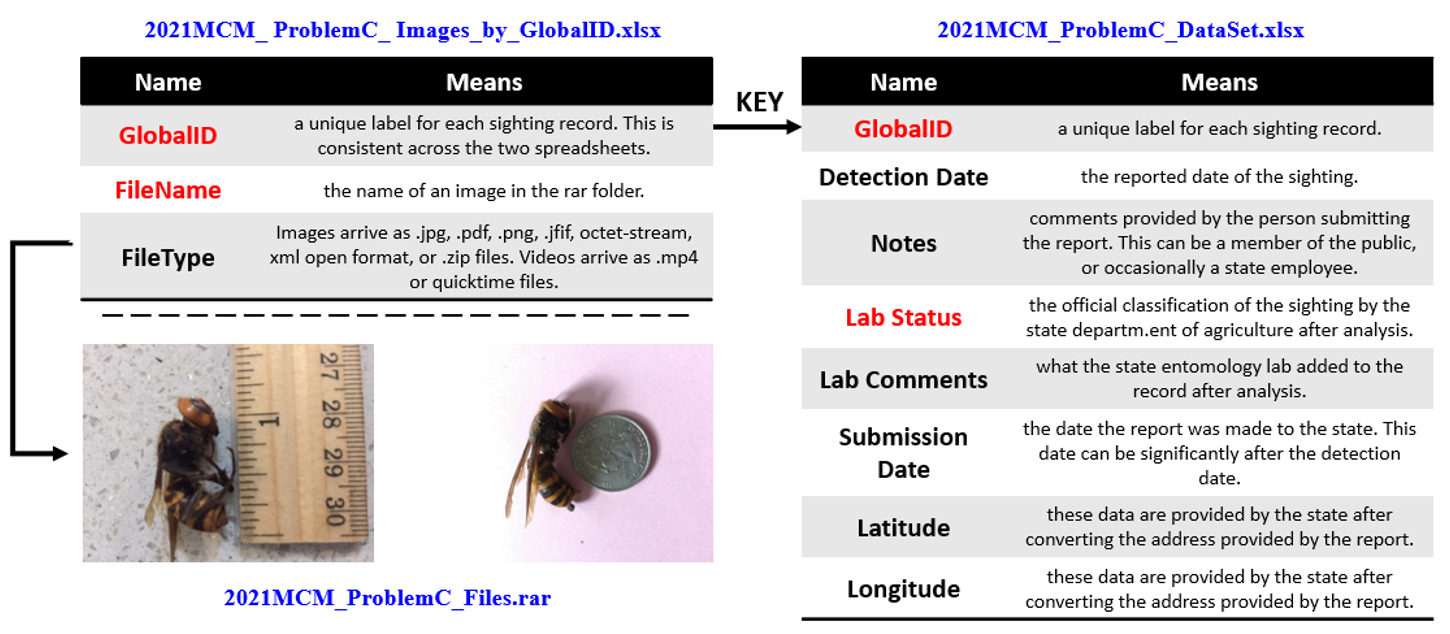
\includegraphics[width=\textwidth]{screenshot010}
	\caption{The relationship each data set, the red letter represents the key data}
	\label{fig:screenshot010}
\end{figure}


\subsection{Problem 1}
To address and discuss whether the spread of this pest over time can be predicted and to what degree of accuracy, we decided to use multivariate time series analysis with the date of reported sightings as time and the latitude and longitude of the sighting site as bivariate variables.

\hspace*{\fill}
\subsubsection{Data preprocessing}
We analyze the data given in the files and count the number of classified samples of the Lab Status item in 2021 MCM$ \_ $ProblemC$ \_ $DataSet.xlsx, as shown in the following table:

\begin{table}[!htbp]   %[H]
	\centering\caption{Classification Sample Statistics of Lab State }
	\begin{tabular}{ccc}
		\toprule[1.5pt]
	Lab Status&	Means&	Numbers\\
		\midrule[1pt]
Positive ID	&is confirmed as an Asian Giant Hornet.&	14\\
Negative ID &	is excluded	&2070\\
Unprocessed &	 not yet been classified.&	15\\
Unverified	&no determination was made due to lack of information.&	2342\\
		\bottomrule[1.5pt]
	\end{tabular}
\end{table}
The information provided by Positive IDs is worth concerning. 

Considering that the flying distance of the bumblebee is 30km during breeding, we draw their trajectory. From figure(a), we can find that the Global Id of (FC6E894B-F6DF-4FDC-853A-D7372D253988) and (124B9BFA-7F7B-4B8E-8A56-42E067F0F72) are far greater than the effective flight distance of the Hornet. Therefore, we regard them as outlier elimination, and draw revised trajectory diagram of the bumblebee (b).

\begin{figure}[H]
	\centering
	\subfigure{
		\begin{minipage}[t]{0.5\textwidth}
			\centering
			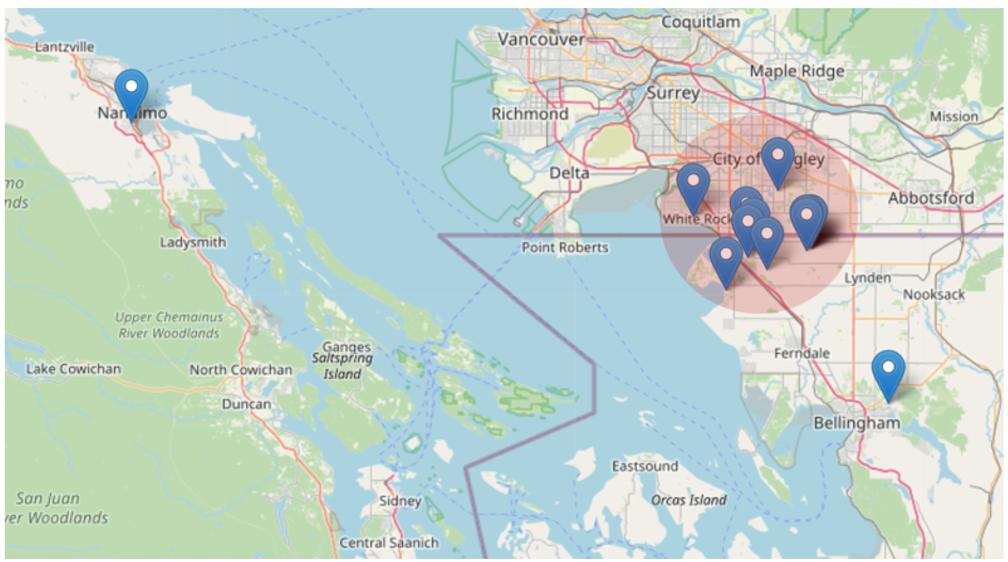
\includegraphics[width=8cm]{screenshot011}
			\caption{(a) represents the effective range of the bumblebee}
		\end{minipage}%
	}%
	\subfigure{
		\begin{minipage}[t]{0.5\textwidth}
			\centering
			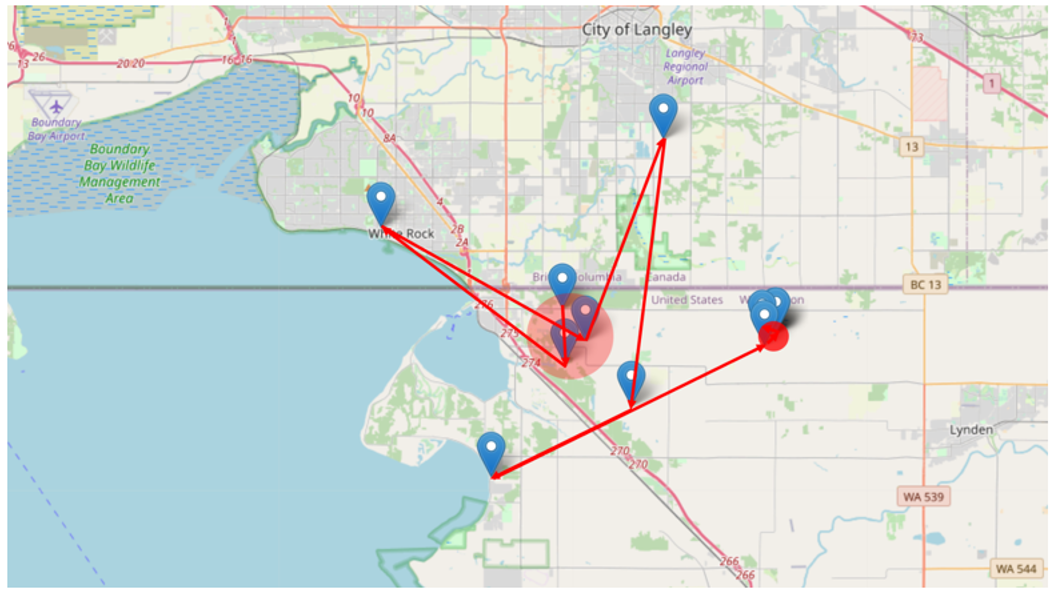
\includegraphics[width=8cm]{screenshot012}
			\caption{(b) represents the trajectory of the bumblebee}
	\end{minipage}}
\end{figure}

Next, we extend the records of Positive IDs.After analyzing the key attribute of Positive IDs and Detection IDs, we find that the interval between detection times is irregular.It is known from  problem literature that the queen bee is inactive in winter. Therefore, we do not supplement the data in winter. For the rest of the data, we fill in the mean interpolation at 15-day intervals. 

The filling formula is as follows:
\begin{equation}
	L^N=L^B+\frac{L^E-L^B}{\frac{h}{15}}
\end{equation}
Part of the expanded data is shown in the following table:

\begin{table}[H]   %[H]
	\centering	\caption{Some examples of expanded data}
	\begin{tabular}{cccc}
		\toprule[1.5pt]
		Detection Date&Latitude&Longitude &	Lab Status \\
		\midrule[1pt]
2019/10/15&	48.98292&	-122.702	&Positive\\
2019/12/1 &	49.00341 & -122.75 &	Positive\\
		\bottomrule[1.5pt]
	\end{tabular}
\end{table}

At the same time, in order to analyze the relationship between a bumblebee's moving position and time, we construct a time series data set. 
And then, we use the former three sets of data to predict the latter one 
The purpose of constructing the data set in this way is to fully consider the feature correlation between the spatial position and time of the bumblebee.

\hspace*{\fill}
\subsubsection{Problem Modeling}
In response to the first question, we constructed a sequence data set of the bumblebee's moving position and time, and at the same time built an LSTM network to capture the relationship between the bumblebee's spatial position and time, and then realized the accurate prediction of the bumblebee's spatial position change. 

The structure of our model is shown in the following diagram:
\begin{figure}[H]
	\centering
	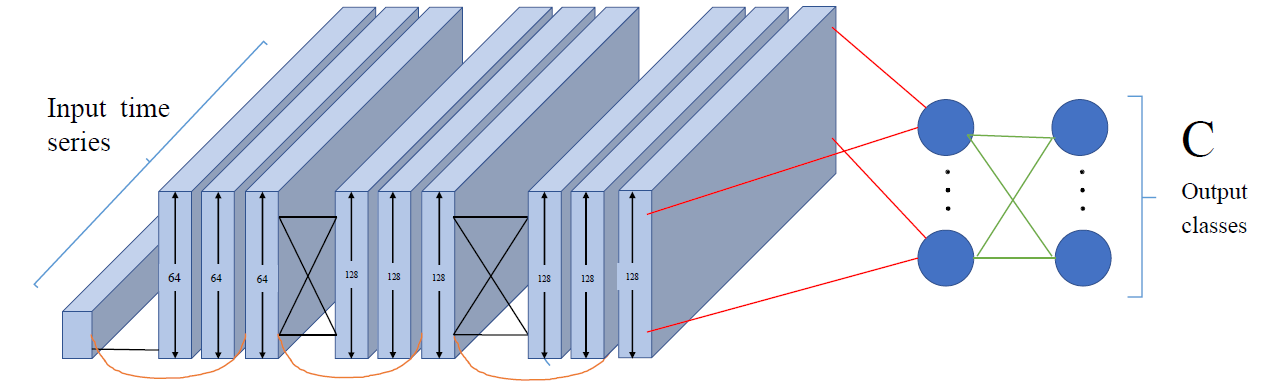
\includegraphics[width=\textwidth]{screenshot008}
	\caption{Residual network's architecture. Black connections correspond to convolutions, orange to residual, red to average pooling and green are fully-connected}
	\label{fig:screenshot008}
\end{figure}

The long short term memory (LSTM) neural network, first proposed in 1997, is a huge improvement for the recurrent neural network (RNN). 

As shown in the figure 5, through selective memory of historical information, LSTM neural network solves the problem of RNN gradient explosion and gradient disappearance. LSTM neural network adds three important gate control functions to the memory unit module of the hidden layer. The three different gate control functions correspond to three different gate control functions, namely input gate, forget gate and output gate. The LSTM neural network controls the storage and transmission of information through three gate functions of the hidden layer memory module.

\textbf{(1) The main role of the forgetting gate} ($ f_t $) is to control the amount of data of the input information and to control the time span of the data consistently by discarding part of the historical information, which is achieved by the Sigmoid activation function and takes values between (0,1). Figure 6 shows the schematic diagram of the forgetting gate structure

The forgetting gate controls the superposition of the hidden layer $ h_{t-1} $ output and the input layer $ x_t $ input by the sigmoid function, and the output $ f_t $ of the forgetting gate is expressed as
\begin{equation}
	f_t=\sigma(W_fh_{t-1}+U_fx_t+V_fc_{t-1}+b_f)
\end{equation}

\textbf{(2) The main role of input gate} (($ t_i $)) is to update the information of the current moment and input the output of the hidden layer of the previous moment into the current moment, so as to achieve the transfer of timing information.Figure 7 shows the schematic structure of the input gate.

\begin{figure}[H]
	\centering
	\subfigure{
		\begin{minipage}[t]{0.5\textwidth}
			\centering
			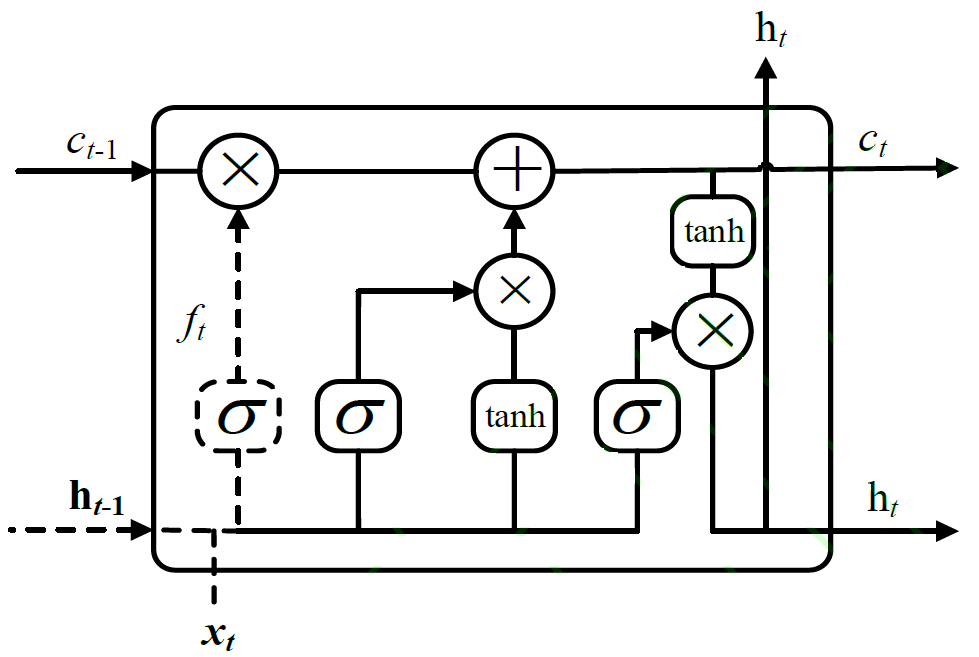
\includegraphics[width=8cm]{tu5.png}
			\caption{The sketch of input gate of LSTM}
		\end{minipage}%
	}%
	\subfigure{
		\begin{minipage}[t]{0.5\textwidth}
			\centering
			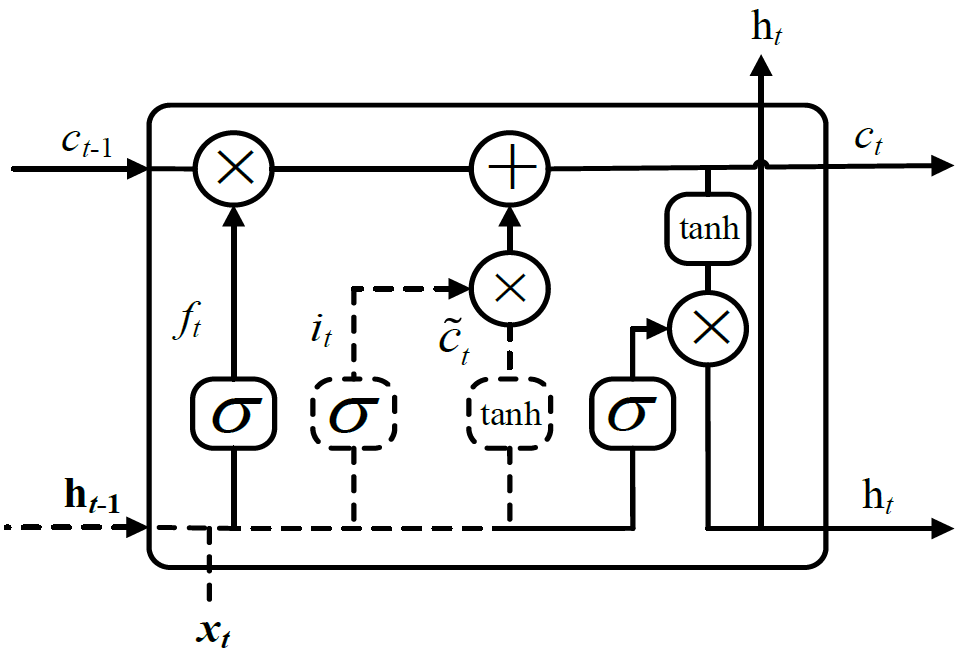
\includegraphics[width=8cm]{tu6.png}
			\caption{The sketch of input gate of LSTM}
	\end{minipage}}
\end{figure}

The process of superimposing the output of the hidden layer at the previous moment with the current input is
\begin{equation}
	i_t=\sigma(W_ih_{t-1}+U_ix_t+V_ic_{t-1}+b_i)
\end{equation}

According to the joint action of the forgetting gate and the input gate, the hidden layer memory cell realizes the information update and outputs the memory cell $ c_t $ , and the hidden layer memory cell is calculated as

\begin{equation}
	c_t= i_t \tanh(U_cx_t+W_ch_{t-1}+b_c)+f_tc_{t-1}
\end{equation}

\textbf{(3) The output gate} ($ o_t $) controls the output information and returns the timing information of the hidden layer through the output gate before the memory cell outputs the information, thus ensuring that the information of the memory cell is updated. The structure of the output gate is shown in Figure 8.

The output gate is calculated as
\begin{equation}
	o_t=\sigma(U_ox_t+W_oh_{t-1}+V_oc_{t}+b_o)
\end{equation}
The method to return the output $ h_t $ of the hidden layer is calculated as
$ h_t=o_t\tanh(c_t) $

\begin{figure}[H]
	\centering
	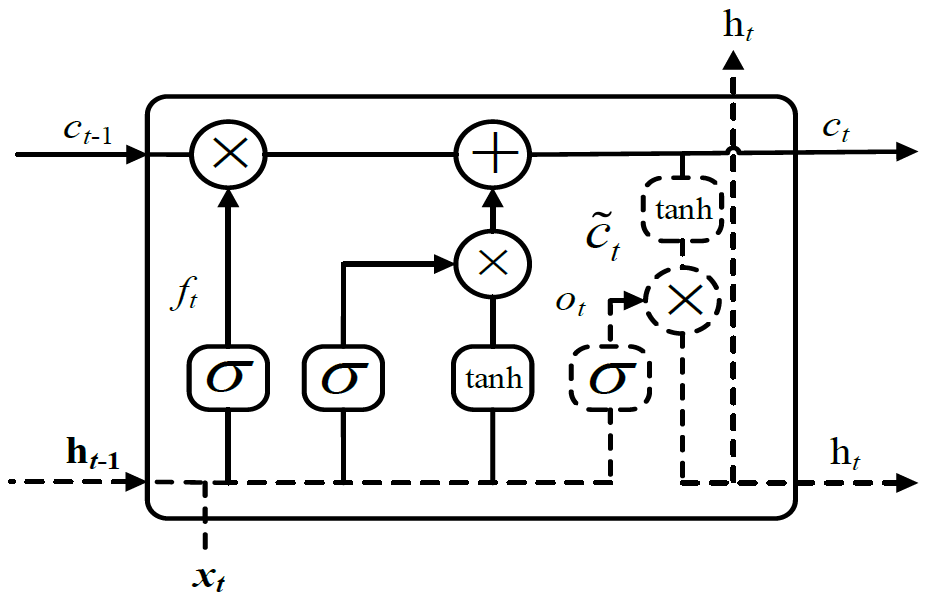
\includegraphics[width=0.45\textwidth]{tu7.png}
	\caption{The sketch of input gate of LSTM}
\end{figure}
\subsubsection{Model solving}
We use the expanded  time series data set about hornet to train the LSTM model. We use  keras library in python to build LSTM to predict the spatial position of the bumblebee. See the appendix for the specific code. First, we set the number of single-layer LSTM units to 32. Then we set the dropout layer to 0.15 to randomly discard $ 15\% $ of the parameters. The batch size for model training is 4 and the epoch is 15. At the same time, Mean Square Error (MSE) is used as the loss function, and Adam is the optimizer.

The calculation formula of MSE is as follows:
\begin{equation}
	MSE=\frac{1}{n}\sum_{i=1}^{n}(\hat{y_i}-y_i)^2
\end{equation}

In the end,after 15 rounds of calculation, the final MSE value of the training set is calculated to be 0.1531. The accuracy rate reached $ 66.7\% $. This means that our model can predict the spatial position of the wasp.

\hspace*{\fill}
\subsubsection{Conclusion}
After using the LSTM model, the prediction accuracy rate reaches more than $ 60\% $. This model can be used to predict the spatial position of the wasp.

\hspace*{\fill}
\subsection{Problem 2}

\subsubsection{Data preprocessing}
We first identify the Global ID as the key factor in the process of connecting simultaneous image and label data tables, and then perform an overview analysis of the data.The key data items are shown in the table below:
\begin{table}[H]   %[H]
	\centering	\caption{Data overview table}
	\begin{tabular}{ccc}
		\toprule[1.5pt]
Name &	Images Numbers	&GlobalID Numbers\\
		\midrule[1pt]
PositiveId&	14&	11\\
NegativeId&	3194&	2126\\
Unprocessed &11	&-\\
Unverified	&86&	-\\
		\bottomrule[1.5pt]
	\end{tabular}
\end{table}

It can be seen from the files that the number of image samples of non-hornets is much more than that of hornets. In deep learning, for  avoiding overfitting, we should input sufficient data. So we first increase the number of bumblebee image samples.

Considering that the bumblebee image contains  redundant data, we cut the bumblebee image to ensure that the data redundancy  after data enhancement is less in advance.The examples of image cropping processing are shown below:
\begin{figure}[H]
	\centering
	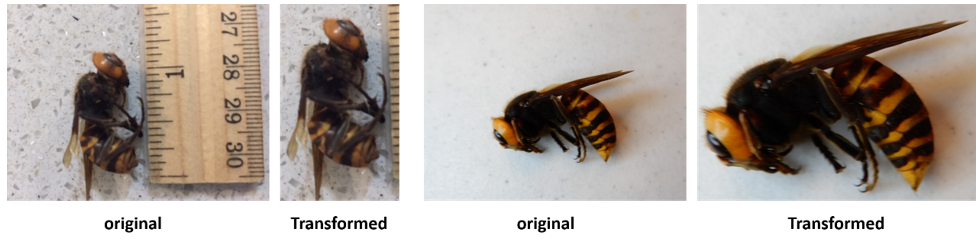
\includegraphics[width=0.8\textwidth]{screenshot014}
	\caption{cropping example}
	\label{fig:screenshot014}
\end{figure}

We enhance the accuracy of the data by using the following methods:

\begin{itemize}
	\item \textbf{Rotation:} Randomly rotate the image to a certain angle; change the orientation of the image content;
	\item \textbf{Flip:} Flip the image along the horizontal or vertical direction;
	\item \textbf{Zoom:} Zoom in or zoom out the image according to a certain ratio;
	\item \textbf{Shift:} The image is translated in a certain way on the image plane;
	\item \textbf{Scale:} The image is enlarged or reduced according to the specified scale factor. Change the size or blur degree of the image content;
	\item \textbf{Contrast transformation: }In the HSV color space of the image, the saturation S and V brightness components are changed, and the hue H remains unchanged. Exponential operations are performed on the S and V components of each pixel to increase the illumination change.
	\item \textbf{Noise:} Randomly perturb each pixel RGB of the image, we use Gaussian noise.
\end{itemize}

We transform each image 40 times, and the transformed image output is shown in the following figure:
\begin{figure}[H]
	\centering
	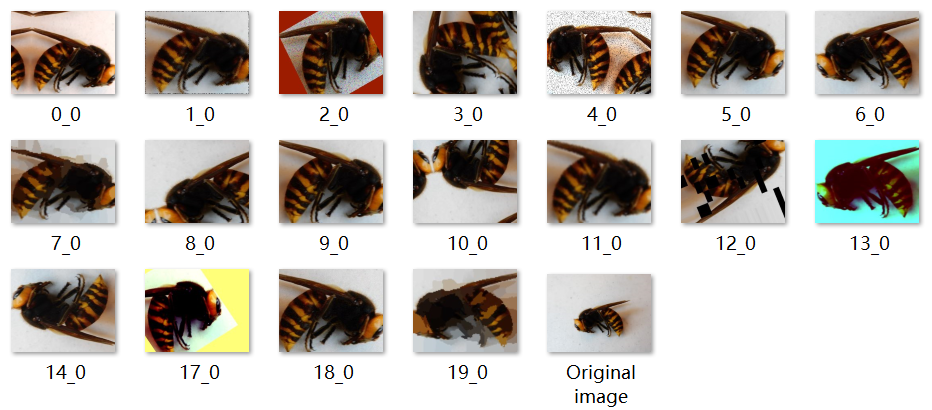
\includegraphics[width=0.8\textwidth]{screenshot013}
	\caption{Transformation result output}
	\label{fig:screenshot013}
\end{figure}

At the same time, too many non-bumblebee samples are easy to cause data redundancy.This redundancy can also happen because the images provided by the same Global ID are too similar.Therefore, if there are multiple images in a global ID, we will randomly select one of the images for subsampling to ensure the balance of positive and negative samples.

\hspace*{\fill}
\subsubsection{Problem Modeling}
In the second question, considering that  samples is few in number, we combine the knowledge of transfer learning and use the VGG19 pre-trained convolutional neural network to perform transfer learning. The model structure is shown in the figure below:

\begin{figure}[H]
	\centering
	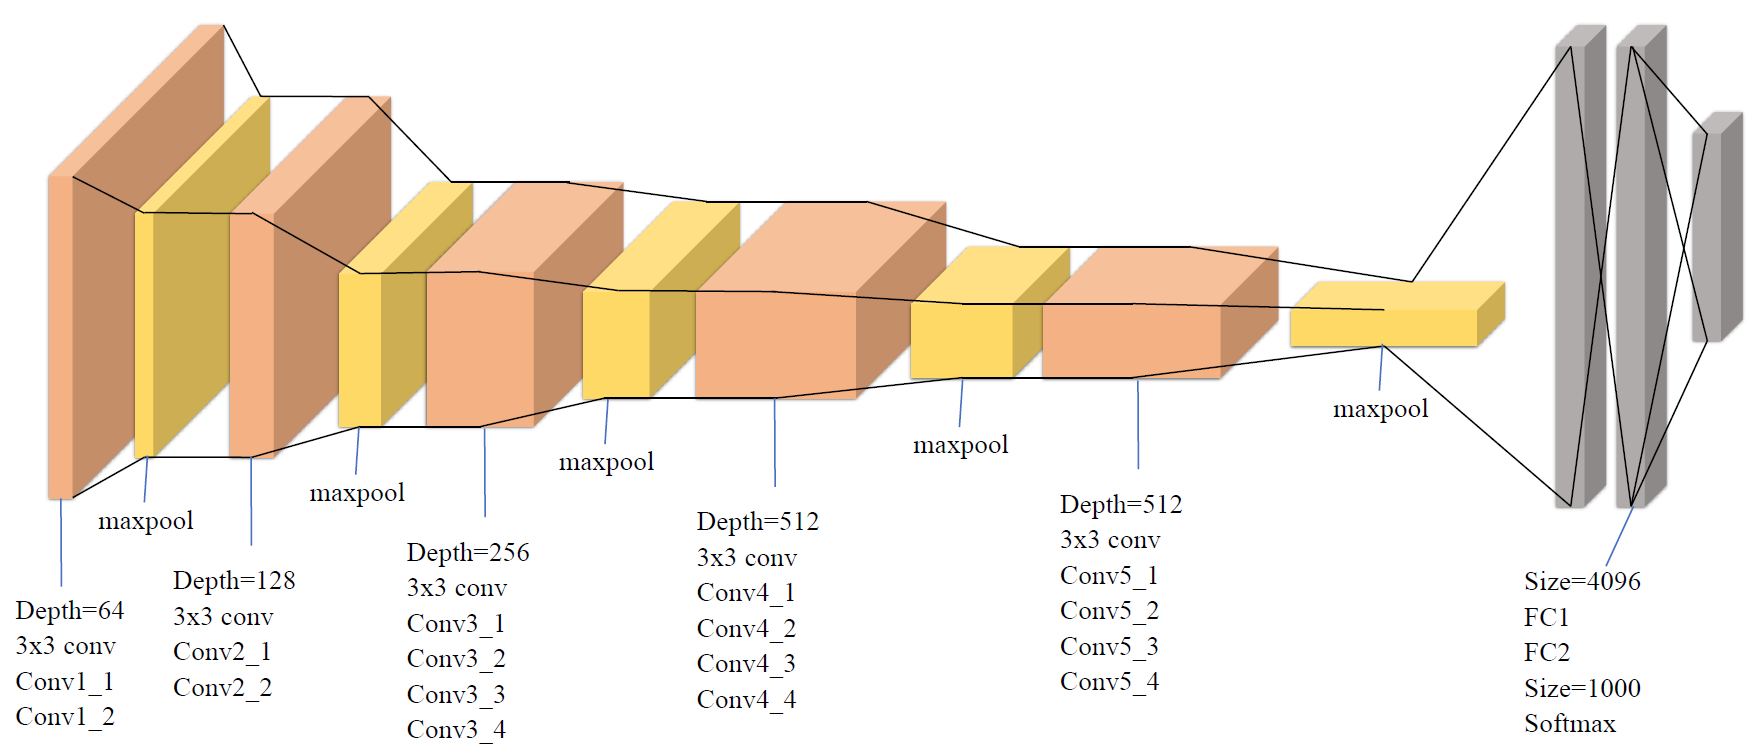
\includegraphics[width=\textwidth]{screenshot009}
	\caption{VGG-19 Model Architecture}
	\label{fig:screenshot009}
\end{figure}

Transfer learning is a machine learning method that can apply knowledge learned from other fields to the required research field. When a neural network is trained, it is generally considered that the training set and the test set are the same distribution, and thousands of samples are needed to train and optimize the model. Therefore, even if the samples are sufficient, processing the sample data is a costly process; and the transfer learning method can well make up for the problems caused by insufficient data or excessive training time.

The VGG16 convolutional neural network is a process of extracting and continuously refining images, and it has a deep network structure.At first, the convolutional layer only extracts the features of the image, and only when the network layer is deeper can it deal with specific tasks. Therefore, in the migration learning process, the model that has been pre-trained in the source domain can be used, the weight of the lower layer is retained, and only the upper layer is retrained and related parameters are fine-tuned. Because of the different characteristics of the source domain data distribution, it is necessary to use the target domain dataset to fine-tune the model, remove the original top layer and add a new output layer, and add the softmax function to classify the new problem. Figure 12 shows a process of migrating the model. By migrating the weights trained in the source domain (natural image) in the model, and then using the target domain (task data) for fine-tuning, it greatly simplifies the model in the new domain. 

\begin{figure}[H]
	\centering
	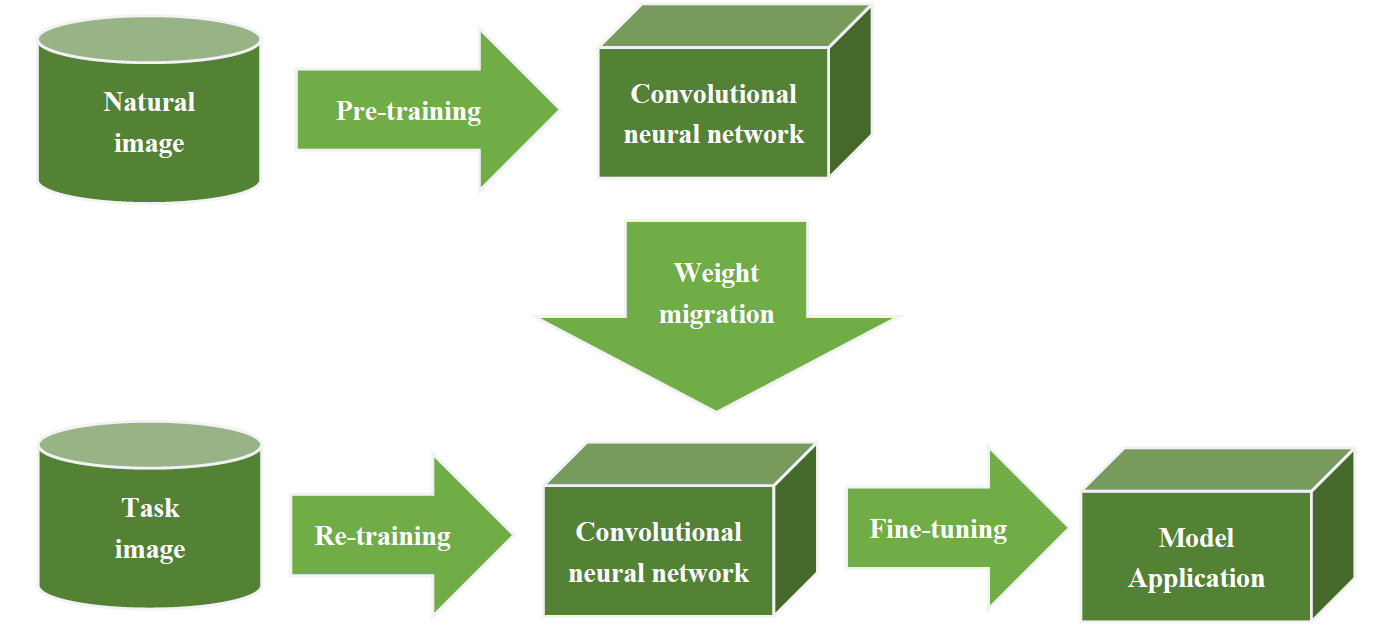
\includegraphics[width=0.8\textwidth]{screenshot006}
	\caption{Model transfer of CNN}
	\label{fig:screenshot006}
\end{figure}
%\begin{figure}[H]
%	\centering
%	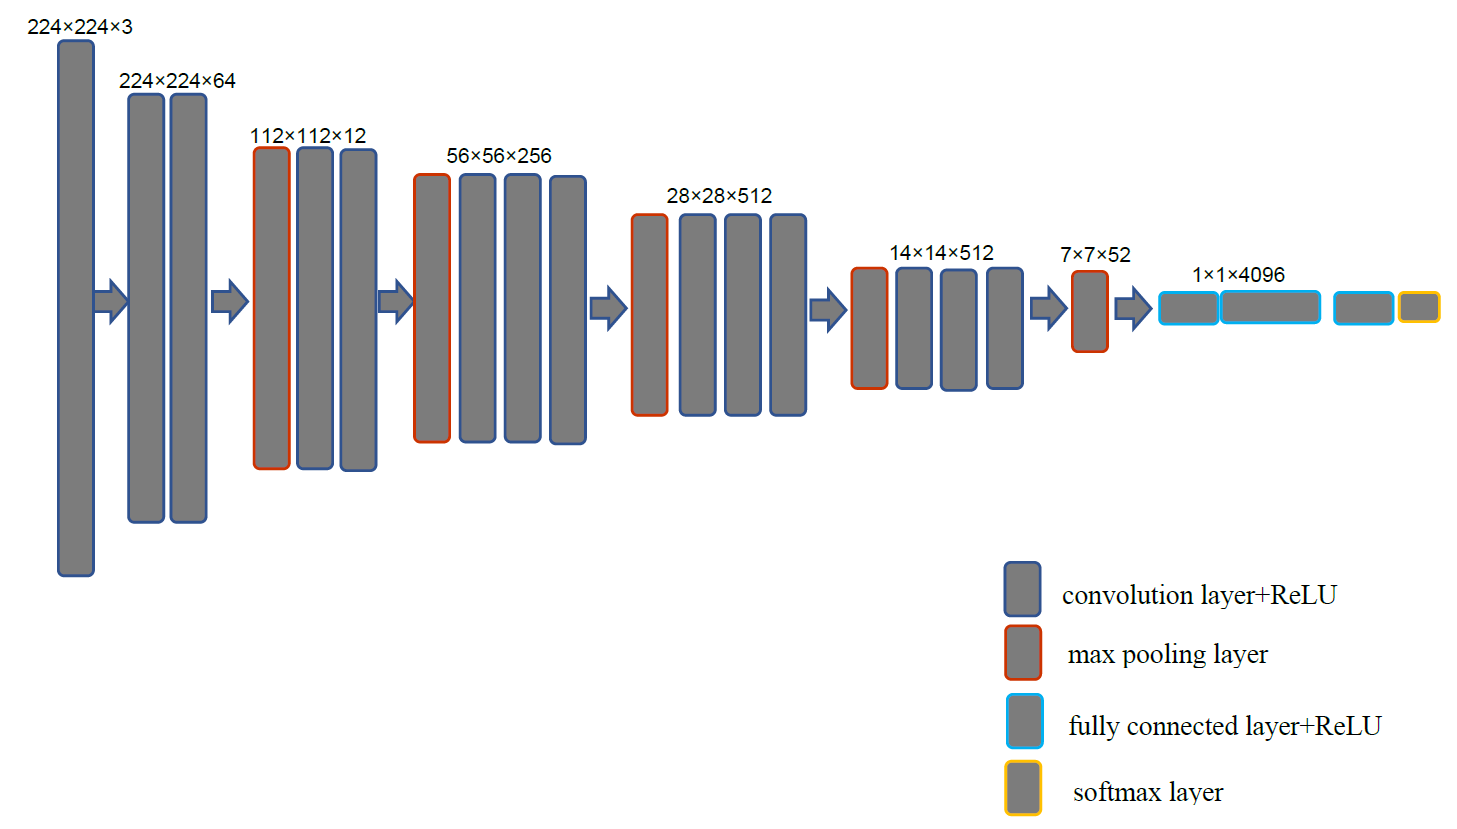
\includegraphics[width=\textwidth]{screenshot007}
%	\caption{Structure chart of VGG16 convolutional neural network}
%	\label{fig:screenshot007}
%\end{figure}

\subsubsection{Model solving}
The new data set after data enhancement is used to train the convolutional neural network for image recognition of bumblebee. We use the VGG19 model pre-trained on imagenet. However, our training strategy is fine-tune. Specifically, we freeze the parameters of the first fifteen layers of networks, and then retrain the models after fifteen layers. It ensures that a better effect can be achieved on small data sets.

We divide the data set into training set and test set according to 8:2. 
When the batch size is set to 32 and the learning rate is 1e-4, 20 epochs are trained. At the same time, we use the binary cross entropy loss function, the formula is as follows:
\begin{equation}
	L_{logistic}(\hat{y}-y)=-y\log\hat{y}-(1-y)\log(1-\hat{y}),\; y\in\left\lbrace 0,1\right\rbrace
\end{equation}

$ \hat{y}=\sigma(\bar{y}) ,\;\; \sigma(\bar{y})=\frac{1}{1+e^{-\bar{y}}}  ,\;\; \frac{\partial \sigma}{\partial \bar{y}}=\sigma(1-\sigma)  ,\;\; \bar{y}=w\cdot x +b=\sum_{j}w_jx_j+b ,\;\; \frac{\partial \bar{y}}{\partial w_j}=x_j $

During the model training process, we draw the test set , training set loss and accuracy change curve. They are in the figure 13.

It can be seen that after the 8th epoch, the accuracy of the model on the test set basically does not change. Meanwhile, the model reaches a state of convergence. At this time, the accuracy on the test set is $ 92.7\% $. 
This strongly proves the effectiveness of our data enhancement strategy and the precise identification of bumblebees.

Besides,we also use multiple evaluation indicators such as F1 score 、precall and recall  to test the error rate of the model. 

\begin{figure}[H]
	\centering
	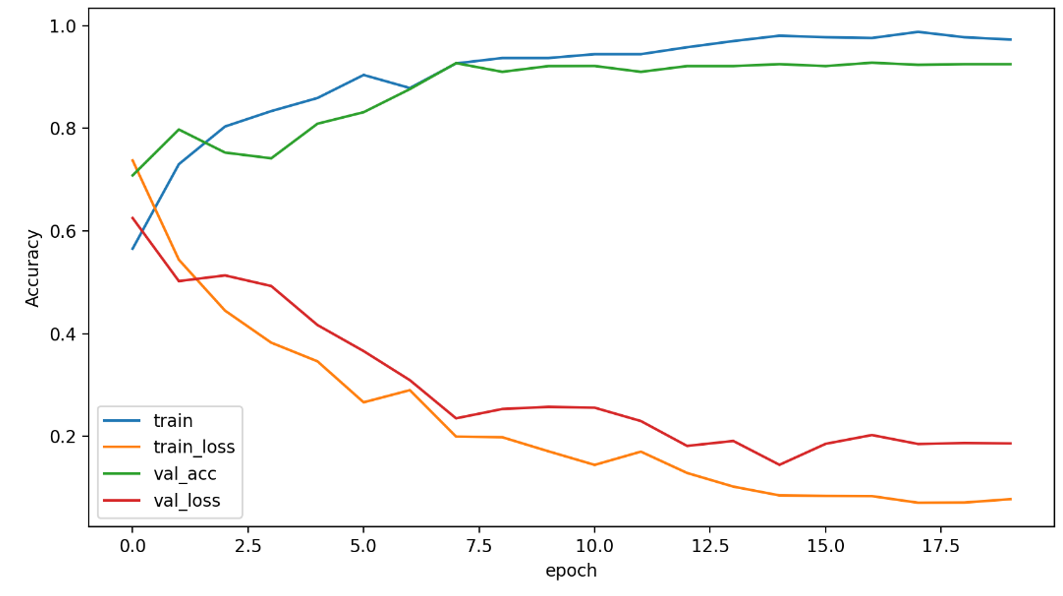
\includegraphics[width=0.8\textwidth]{screenshot018}
	\caption{Change curve of training set loss and accuracy}
	\label{fig:screenshot018}
\end{figure}

The relevant calculation formula is as follows:
\begin{equation}
	Accuracy=\frac{TP+TN}{TP+TN+FP+FN}
\end{equation}
\begin{equation}
	Precall=\frac{TP}{TP+FP},\;Recall=\frac{TP}{TP+FN}
\end{equation}
\begin{equation}
	F1=\frac{2\times Precall\times Recall}{Precall+Recall}
\end{equation}

The final model's performance test results for each indicator on the test set were accuracy rate 0.927, precall: 0.893, recall: 0, 915, and F1 score: 0.903.

\hspace*{\fill}
\subsubsection{Conclusion}
From the results, the model can be used to determine whether the bee species witnessed by the eyewitness is the target bee species.

\hspace*{\fill}
\subsection{Problem 3}
\subsubsection{Data preprocessing}
In the modeling of question three, we comprehensively considered the image information and text information of each event to establish an event quick response model to detect whether the unprocessed and unprocessed data contains bumblebee-related information.

We first filter the data whose Lab Status is negative and positive, and then use the jieba module in python for word segmentation of the text in their note attributes, and use wordcloud to draw their respective word clouds for data overview. 
The cloud is shown below:
\begin{figure}[H]
	\centering
	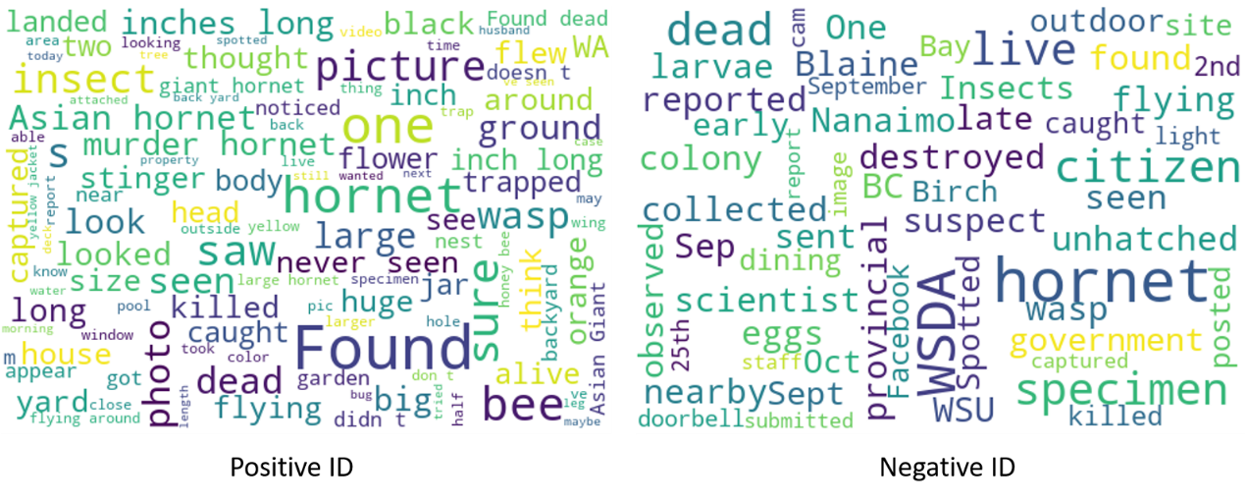
\includegraphics[width=\textwidth]{screenshot015}
	\caption{High-frequency word cloud image}
	\label{fig:screenshot015}
\end{figure}

Then we calculated the 50 most frequent words in negative, and the word frequency distribution diagram is as follows:

\begin{figure}[H]
	\centering
	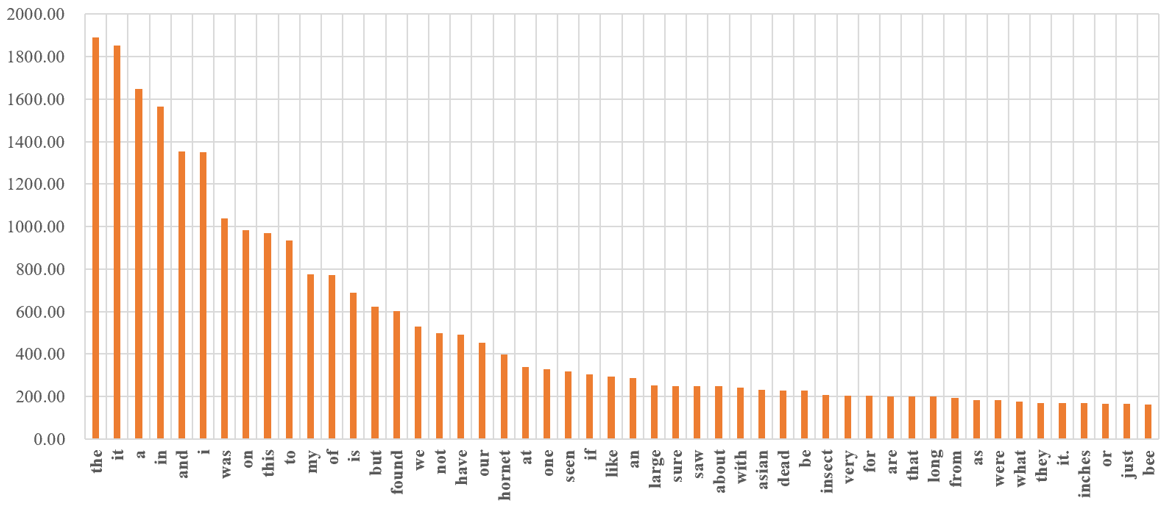
\includegraphics[width=\textwidth]{screenshot016}
	\caption{Word frequency distribution map}
	\label{fig:screenshot016}
\end{figure}

We compose a new string of the fifty most frequently occurring words as a negative dictionary string, and compare the similarity of the note text in other records with it during model building. The samples with high similarity are considered to be negative samples, and the samples with low similarity are considered to be positive samples. The specific model design and threshold selection are explained below.

\subsubsection{Problem Modeling}
Under the premise of limited manpower and material resources, in order to quickly judge the right or wrong of eyewitness reports, we built a time quick response model as shown in following figure:

\begin{figure}[H]
	\centering
	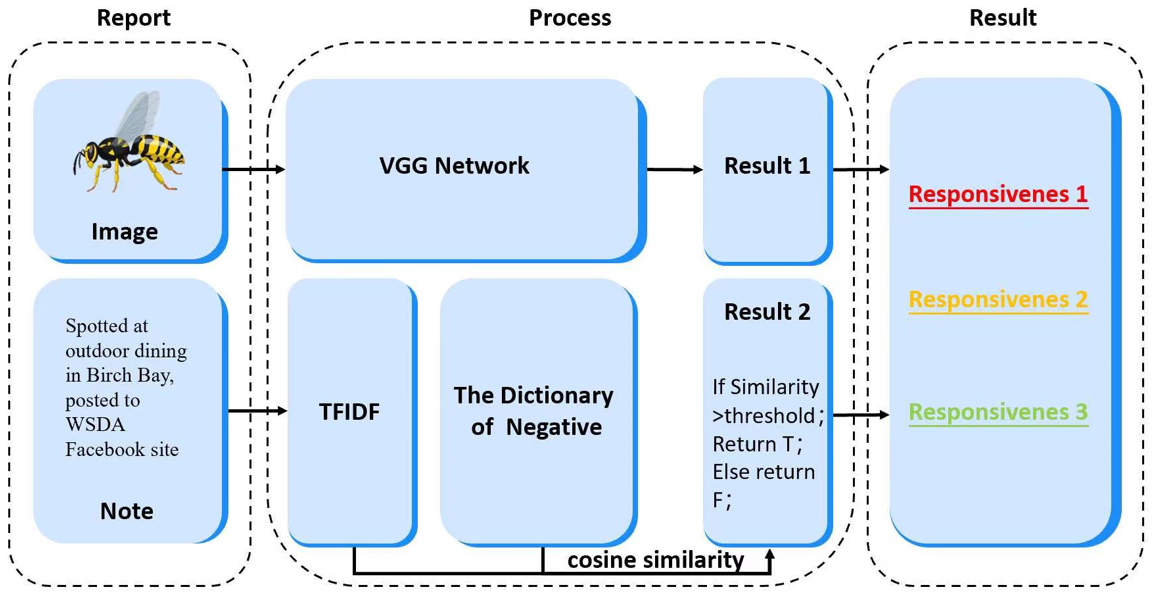
\includegraphics[width=\textwidth]{screenshot017}
	\caption{The structure diagram of the rapid response model}
	\label{fig:screenshot017}
\end{figure}

In the model, we use TF-IDF (term frequency—inverse document frequency) to extract word vectors. Tfidf is a commonly used weighting technique for information retrieval and data mining. TF is Term Frequency, and IDF is Inverse Document Frequency. It is used to evaluate the importance of a word to a document set or a document in a corpus. The importance of a word increases in proportion to the number of times it appears in the document, but it decreases in inverse proportion to the frequency of its appearance in the corpus.

We also use the cosine distance to calculate the similarity between strings. The cosine similarity calculation formula is as follows:
\begin{equation}
	similarity=cos(\theta)=\frac{A\cdot B}{||A||\;||B||}
\end{equation}
A and B represents two word vectors in our model.

Specifically, when the wasp image detection model in problem two determines that the image contained in a certain report is a wasp, we will also judge the similarity between the note contained in this report and the negative dictionary string. Combining image recognition results and similarity, we designed a three-level response, as shown below:
\begin{itemize}
	\item \textbf{First-level Response:} When the image and similarity both reach the threshold , we define it as the first-level response (that is, the report that should be processed first, most likely a bumblebee)
	\item \textbf{Second-level Response:} When either the image or the similarity reaches the threshold, we define it as the secondary response (that is, the report corresponding to the priority processing, which may be a bumblebee)
	\item \textbf{Third-level response:} When the image and similarity does not reach the threshold, we define it as a three-level response (that is, the report that does not need to be processed immediately, very unlikely a bumblebee)
\end{itemize}

The design of model threshold value will be given in detail in the problem solving.

\hspace*{\fill}
\subsubsection{Model solving}
In the process of solving the fast response model, the key value is the text similarity threshold.We compare the similarity between positive text and negative dictionary strings . We also compare the similarity between negative text and negative dictionary strings. Consequently, we  find that the former is much less similar than the latter.

\begin{table}[H]   %[H]
	\centering\caption{Similarity statistics table}
	\begin{tabular}{ccc}
		\toprule[1.5pt]
GlobalID&	Lat status&	Similarty\\
		\midrule[1pt]
{5AC8034E-5B46-4294-85F0-5B13117EBEFE}&	Positive ID	&0.371\\
{2138197A-F5CF-4308-93E2-62EA6F84D098}&	Positive ID	&0.155\\
{DEF5D82B-E326-41A5-9B6CD46DCD86950C}&	Positive ID	&0.225\\
{C4F44511-EA53-4FCF-9422-E1C57703720D}&Negative ID&	0.894\\
{89C867F1-D5ED-48C8-9586-B705F5DA9838}&Negative ID&	0.768\\
{81670D96-4143-47B1-A9C8-83977892D53F}&	Negative ID	&0.882\\
{D30895B7-3994-45A3-BD51-E5BA881833FD}&Negative ID	&0.813\\
		\bottomrule[1.5pt]
	\end{tabular}
\end{table}

Through the table 4, we can clearly see the effectiveness of the similarity comparison. Taking into account the number of Positive IDs given in the question, we set the threshold to the mean value of the similarity of each Positive ID containing notes. We calculate the mean value of similarity of each Positive ID: 0.287. So the text similarity threshold is solved as 0.287.

After obtaining the threshold of the model, we filter out the unprocessed and unverified data and send it to the model to determine its response degree. Some of the first and second response degree reports are shown below.
\begin{table}[H]   %[H]
	\centering\caption{Responsibility judgment result table}
	\begin{tabular}{cccc}
		\toprule[1.5pt]
GloballID&	image&	Simlarty&	Responsiveness\\
		\midrule[1pt]
{AE7F3E03-F339-4081-8D83-CFCBC8B9DAA9}&	T&	0.268&	1\\
{3E50801D-9DBB-43DE-8D32-31CFA88C74D9}&	T&	0.253&	1\\
{BBBA5BA0-CAFB-43D3-8F1D-FB2D9CF777E0}&	T&	0.847&	2\\
{41EB9554-6676-4CD1-BE5B-5133CB3EE4B0}&	T&	0.687&	2\\
{016DDF49-2218-4073-A5F4-32396D0D4B70}&	T&	0.777&	2\\
		\bottomrule[1.5pt]
\end{tabular}
\end{table}

The pictures corresponding to the first and second level reports of unprocessed and unverified data are as follows:

\begin{figure}[H]
	\centering
	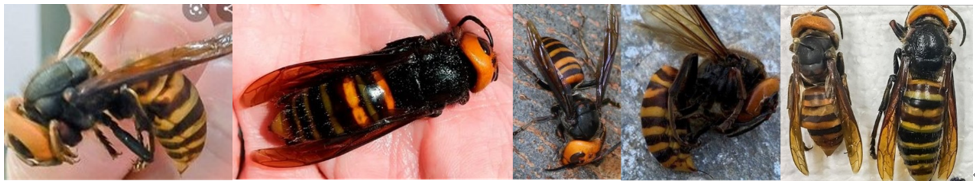
\includegraphics[width=0.7\textwidth]{screenshot019}
	\caption{The picture corresponding to the report of the first and second response levels}
	\label{fig:screenshot019}
\end{figure}

\subsubsection{Conclusion}
From the model results , the model can be used as the credibility of whether the bee is an Asian giant hornet through the similarity and response degree .

\hspace*{\fill}
\subsection{Problem 4}

\subsubsection{Data preprocessing}
Through consulting the literature and analyzing the information provided by this subject, we know that the appearance of wasps has obvious seasonal changes.Data show that the high frequency period of Asian bumblebee is from May to August.Other similar species of bees appeared around this time.This will lead to an increase in the number of reports.To better determine the frequency of model updates, we will first count the frequency of reports and the relationship between the months.

The data given contains a lot of invalid date information, while the month and season factors are important information that needs attention. For more detailed analysis, we clean the invalid date data and combine the number of reports appearing in the same month in different years as well. 
The relationship between the frequency of report and the month is shown in the following table:

\begin{table}[H]   %[H]
	\centering	\caption{Frequency statistics in different months}
	\begin{tabular}{cccccc}
		\toprule[1.5pt]
Month & Reports & Negative & Positive & Unprocessed & Unverified \\
		\midrule[1pt]
		1     & 6       & 2        & 0        & 0           & 4          \\
		2     & 5       & 3        & 0        & 0           & 2          \\
		3     & 23      & 5        & 0        & 0           & 18         \\
		4     & 194     & 44       & 0        & 0           & 150        \\
		5     & 581     & 129      & 2        & 0           & 450        \\
		6     & 342     & 187      & 1        & 0           & 154        \\
		7     & 1028    & 542      & 0        & 0           & 486        \\
		8     & 1396    & 715      & 1        & 6           & 674        \\
		9     & 660     & 353      & 6        & 2           & 299        \\
		10    & 183     & 87       & 2        & 7           & 87         \\
		11    & 5       & 0        & 1        & 1           & 3          \\
		12    & 3       & 0        & 1        & 0           & 2         \\
		\bottomrule[1.5pt]
	\end{tabular}
\end{table}
\subsubsection{Problem Analysis and Modeling}
In this problem, we need to figure out the update frequency of the model. First, we consult relevant literature and learn that the deep learning model used in Question 2 requires a large amount of computing resources and data.  Nevertheless, the real world situation is  more complicated and changeable. So outdated models often fail to achieve excellent results. Based on the above reasons, we have the most significant principle of our model updating: to update the model as quickly as possible under the premise of ensuring the effective data volume.

From the relationship between the frequency of the report in the data preprocessing section and the month, we can see that the report is concentrated in April to October, which also corresponds to the habitable month of the wasp. Simultaneously, the relationship between frequency and month fits the Gaussian normal distribution function. 
The figure is following below:

\begin{figure}[H]
	\centering
	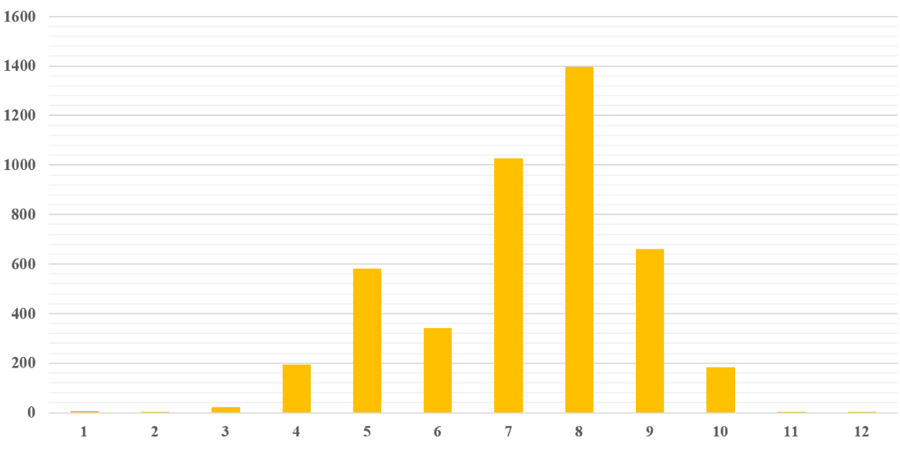
\includegraphics[width=0.8\textwidth]{screenshot020}
	\caption{Frequency and monthly statistics}
	\label{fig:screenshot020}
\end{figure}

From the figure we can see that the report often peaks between August and September. 
A large number of reports correspond to a large amount of data, which can satisfy the training of our model. 

\hspace*{\fill}
\subsubsection{Conclusion}
We conclude that our model should be updated between August and September each year, and the update frequency should be once a year. It can not only ensure the timeliness of the model, but can also satisfy the data amount required by model training.

\hspace*{\fill}
\subsection{Problem 5}
According to the conclusions of questions 1 to 4, the criteria for determining the pests are determined as follows: after the sighting report is updated, the new data is determined by the model to no longer have the primary and secondary responses, indicating that Washington State has got rid of the pest haze.

%-----------------------------------------------------------------------------
\section{Strengths and Weaknesses}
\subsection{Strengths:}
\begin{itemize}
	\item In the modeling of the second problem, we use the method of data augmentation to compensate for the imbalance of positive and negative samples. On this basis, we propose a wasp image recognition model derived on a convolutional neural network. Compared with traditional MLP, convolutional neural network weight sharing in the convolutional layer in CNN reduces the number of trainable parameters in the network and the complexity of the network model. It also has a less overfitting phenomenon. Therefore, it obtains a better generalization ability. 
	
	At the same time, the pooling operation used in CNN significantly reduces the number of neurons in the model and is more robust to the translation of the input space. 
	
	In addition, the introduction of migration learning allows our model to achieve better classification results on small data sets.
	
	\item We propose a set of artificial intelligence-based wasp governance systems in our memo of advice to the Washington government.
	\item In the third question, we comprehensively consider the multi-modal information of text and image. Consequently, we advocate a rapid response model based on multi-modal information. This model comprehensively considers the text and image information in the report. Compared with using only a single modal information, our model builds three response levels based on the results of multi-modal information feedback in order to respond to the report more objectively.
	
\end{itemize}

\hspace*{\fill}
\subsection{Weaknesses:}
\begin{itemize}
	\item The wasp spatial position prediction model in the first model uses less data for training. In contrast, if there is enough data, the LSTM-based wasp spatial position prediction model will achieve better results.
	\item Although the wasp image recognition model based on the convolutional neural network in model two has achieved good results in the field of identifying wasps, the convolutional neural network itself requires higher computer resources and longer training time than traditional methods.
\end{itemize}

\newpage
\section{Memorandum}
\begin{figure}[H]
	\centering
	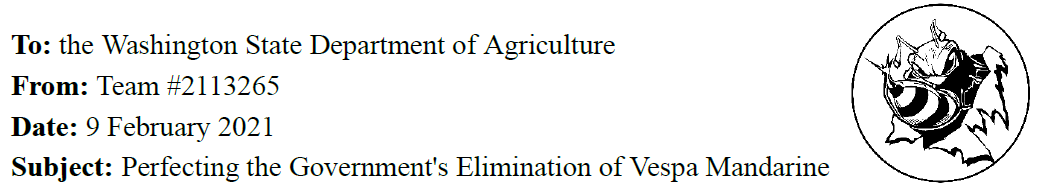
\includegraphics[width=\textwidth]{screenshot023}
\end{figure}
Dear the Washington State Department of Agriculture:

It is our honour to help you formulate policies on Vespa Mandarine to actively respond to pest control. In order to facilitate you to carry out more accurate investigations and protect local biodiversity and social ecological stability, we are very willing to share our modeling results and attach some related policy recommendations based on the models.

We build a three-part model . The first part of the model predict the spread of Vespa mandarine in Washington State over time . The latter two parts of the model establish a three-level response mechanism for public reports by processing image and text data . This mechanism can assess unprocessed sighting reports on three response levels . The results of the response level can be used as the basis of you to formulate the report investigation priority .In the process of building the model, we analyze the seasonal data to determine the active season of the bee colony , which is used to determine the degree of control work carried out at different times .
In order to eliminate pests and reduce the serious impact of species invasion on the ecology and economics of the western United States, we throw out the following six suggestions:

\textbf{1  } We use the model to predict the spread of Vespa Mandarine over time and assess the risk level of being affected by pests under natural environmental conditions. It is recommended that the forecast ranges and statistics provided here be used in conjunction with the pest response guidelines issued by the United States Department of Agriculture so that state governments at all levels can develop strong control strategies.

\textbf{2  }  We use the model to judge the reports that have not yet been determined and not yet processed. In 2344 cases, it is determined that there are five reports with higher response levels. Two of them were first grade and three were second grade. We believe that these five reports are likely to be potential positive IDs. It is recommended that the five ones should be given priority. Careful monitoring and investigation should be carried out within two kilometers of the reported location, and the location of the nests should be tracked by hormones and other biological means for the pests that are found. Do not forget to destroy their nests.

\textbf{3  }  Optimize existing websites and platform hotlines for collecting public reports and improve the standardization and accuracy of collected data, so as to regulate and improve the accuracy of these public reports.

\textbf{4  } In May of each year, use the model to evaluate the new sighting report, as well as use the grade result determined by the model as the basis for the investigation. May is the most active period in the life cycle of the swarm. You can find the nest of Vespa Mandarine more efficiently and eliminate it before expanding the scale of development.
⑤ After a certain number of new Positive IDs are obtained through the above work, they are imported into the model as new basic data for analysis. This approach can get a more accurate prediction map.

\textbf{5  } We evaluate the pest risk level in Washington State through the model. We believe that if you update the data, the new sighting report is judged by the model and no longer has the primary and secondary responses, indicating that Washington State has got rid of the pest haze.

We believe that the model and data we provide will contribute to the response to this species and provide help for the rapid assessment of the priority of numerous public reports in the future. We hope that our model can perfect the government's elimination of pests reducing people's panic as well as returning the natural ecology of Washington State to its original state. So that's the summary of our study. We sincerely hope that it will provide you with useful information. Thank you very much!

%===============================参考文献==============================%

\newpage
\begin{thebibliography}{99}
\bibitem{1} Aversano L , Bernardi M L , Cimitile M , et al. Tomato diseases Classification Based on VGG and Transfer Learning[C]// 2020 IEEE International Workshop on Metrology for Agriculture and Forestry (MetroAgriFor). IEEE, 2020.
Publishing Company , 1984-1986.
\bibitem{2}Yang F W , Lin H J , Yen S H , et al. A Study on the Convolutional Neural Algorithm of Image Style Transfer[J]. International Journal of Pattern Recognition and Artificial Intelligence, 2018.
\bibitem{3}Jing L P , Huang H K , Shi H B . Improved feature selection approach TFIDF in text mining[C]// International Conference on Machine Learning $ \& $ Cybernetics. IEEE, 2002.
\bibitem{4}Van Lenteren J C , Woets J . Biological and integrated pest control in greenhouses.[J]. Annual Review of Entomology, 1988, 33(1):239-269.
\bibitem{5}Gers, Felix A , Schmidhuber, et al. Learning to Forget: Continual Prediction with LSTM.[J]. Neural Computation, 2000.
\bibitem{6}Zheng Z , Ahn S , Chen D , et al. Freeway traffic oscillations: Microscopic analysis of formations and propagations using Wavelet Transform[J]. Transportation Research Part B, 2011, 45(9):1378-1388.
\bibitem{7}Risch S J , Andow D , Altieri M A . Agroecosystem Diversity and Pest Control: Data, Tentative Conclusions, and New Research Directions[J]. Environmental Entomology, 1983, 12(3):625-629.
\bibitem{8}Jianping Ju,Hong Zheng,Xiaohang Xu,Zhongyuan Guo,Zhaohui Zheng,Mingyu Lin. Classification of jujube defects in small data sets based on transfer learning[J]. Neural Computing and Applications,2021
\bibitem{9}D. Lakshmi,K. Palani Thanaraj,M. Arunmozhi. Convolutional neural network in the detection of lung carcinoma using transfer learning approach[J]. International Journal of Imaging Systems and Technology,2020,30(2).
\bibitem{10}Venkatesan Rajinikanth,Alex Noel Joseph Raj,Krishnan Palani Thanaraj,Ganesh R. Naik. A Customized VGG19 Network with Concatenation of Deep and Handcrafted Features for Brain Tumor Detection[J]. Applied Sciences,2020,10(10).
\bibitem{11}Mindy Ward. Dectes stem borer trapping back on in Missouri[J]. Southwest Farm Press,2021.

\end{thebibliography}
%=============================附录:代码,表格等等======================%
\begin{appendices}
Here are simulation programmes we used in our model as follow.\\
\section{}
\textbf{\textcolor[rgb]{0.98,0.00,0.00}{Python code for image training classification}}
\lstinputlisting[language=Python]{./code/01.txt}

\hspace*{\fill}
\section{}\textbf{\textcolor[rgb]{0.98,0.00,0.00}{Python code for LSTM training}}
\lstinputlisting[language=Python]{./code/02.txt}
\end{appendices}
%====================================================================%
\end{document}
